\documentclass{exam}
\providecommand{\abs}[1]{\lvert#1\rvert}
\providecommand{\norm}[1]{\lVert#1\rVert}
\usepackage[utf8]{inputenc}
\usepackage[spanish, es-nolayout]{babel}		
\usepackage{amsmath}						
\usepackage{amsthm}							
\usepackage{amssymb}						
\usepackage{graphicx} 					
\usepackage{float}						
\usepackage{verbatim}					
\usepackage{url}								
\usepackage{subfig}				 
\usepackage{psfrag}			
\usepackage{multicol}
\usepackage{multirow}
\usepackage[bottom]{footmisc}
\usepackage{bigstrut}
\usepackage{color}
	\definecolor{ceruleanblue}{rgb}{0.16, 0.32, 0.75}
	\definecolor{coolblack}{rgb}{0.0, 0.18, 0.39}
	\definecolor{darkgreen}{rgb}{0.0, 0.2, 0.13}
\usepackage{multirow,hhline}
\usepackage{hyperref}
\hypersetup{
    colorlinks=true,
    linkcolor=black, % Color del enlace interno (por ejemplo, índice)
    urlcolor=black, % Color de los enlaces URL
    citecolor=black, % Color de las citas
}
\usepackage{xcolor}
\usepackage{tikz}



\usepackage{newtxmath}

\usepackage{physics}

\renewcommand{\thefootnote}{\fnsymbol{footnote}}


\pagestyle{headandfoot}					
\headrule 										

\firstpageheader{
\includegraphics[scale=0.2]{/Users/joaquin/Documents/GitHub/Ayudant-as-IO/Imágenes/Logo2.png}}{}{\scriptsize{Departamento de Economía} \\ \scriptsize{Facultad de Economía y Negocios}}
\runningheader{\scriptsize{
\includegraphics[scale=0.2]{/Users/joaquin/Documents/GitHub/Ayudant-as-IO/Imágenes/Logo2.png}}}{\scriptsize Microeconomía II \\ \scriptsize{Primavera 2024}} {\scriptsize{Departamento de Economía} \\ \scriptsize{Facultad de Economía y Negocios}}

\footrule
\footer{}{\scriptsize{P\'agina \thepage\ de \numpages}}{}
\parindent = 0pt
\renewcommand\partlabel{(\thepartno.)}
\renewcommand\thesubpart{\roman{subpart}}


\printanswers  
\renewcommand{\solutiontitle}{\noindent\textbf{Respuesta:}\par\noindent\sffamily}

\begin{document}
\begin{center}

\LARGE{\textbf{Microeconomía II}}

\medskip
\normalsize \textbf{Profesora:} Paola Bordón

\normalsize \textbf{Ayudantes:} Ayelén Sandoval, Diego Undurraga, Joaquín Martínez\footnote[2]{joamartine@fen.uchile.cl}


\medskip
\large{\textbf{Ayudantía 7 - Diferenciación Horizontal y Vertical}}

\end{center}

\tableofcontents

\renewcommand{\thefootnote}{\Roman{footnote}}

\section{Diferenciación de producto}

    \subsection{Comentes}
    \begin{itemize}
    \item[\textbf{a.}] Según los modelos de diferenciación vertical pura la diferencia de precios se deben a una diferencia en los costos marginales de producir bienes de mayor o menor calidad.
    \begin{solution}
        Falso, en los modelos de diferenciación vertical pura aunque no hayan diferencias en los costos de producir bienes de menor o mayor calidad habrá una diferenciación. Esto pues que ante máxima diferenciación las firmas que se juegan relajan la competencia por precios.
    \end{solution}
    \item[\textbf{b.}] La principal diferencia entre los modelos con y sin localización es que en los modelos sin localización los consumidores tienen utilidad de la variedad de productos, mientras que en los modelos con localización el consumidor compra solamente de apenas una marca (1 ordenador, 1 casa, etc).
    \begin{solution}
        Verdadero, cuando vemos Hotelling con diferenciación horizontal estamos utilizando modelos de utilidad discreta.
        
          En estos modelos si existen $J$ alternativas en el mercado, indexados por $j = 1, \ldots, J$ el problema del consumidor $i$ se reduce a elegir el que más le brinde utilidad.
            \[
            \max_{j,z} U_i(x_j, z) \quad \text{sujeto a} \quad p_j + p_z z = y_i.
            \]
            donde:
            \begin{itemize}
                \item $x_j$ son las características de la marca $j$, y el precio es $p_j$.
                \item $z$ es la cantidad de la opción alternativa (outside good) y su precio es $p_z$ (generalmente se normaliza $p_z$ a 1).
                \item La opción alternativa (que se denota como $j = 0$) es la opción de no comprar (lo que implica que se gasta su ingreso disponible en otros bienes).
            \end{itemize}
    \end{solution}
    \item[\textbf{c.}] ¿Cuál es la diferencia entre una diferenciación horizontal y vertical?
    \begin{solution}
        Una diferenciación horizontal refiere distinguirsi explotando diferencias en el producto que no incidan en la calidad del mismo. Esto puede ser estética (autos), sabor (cereales), aroma (perfume), y suele ser ejemplificado como la ubicación de venta del producto.

        Por otro lado una diferenciación vertical hace referencia a un espectro de calidad de un mismo producto. Incluso no teniendo diferentes costos de producción las firmas decidirán hacer productos de distinta calidad para disminuir la competencia.

        Ambas suelen tener un mismo resultado, las empresas prefieren diferenciarse para relajar la competencia y acaban obteniendo beneficios positivos aun cuando compiten por precios.
    \end{solution}
    \item[\textbf{d.}] Al diferenciarse horizontalmente el producto nunca cambia. 
    \begin{solution}
        Falso. La diferenciación horizontal cambia características del producto. Por ejemplo estos dos modelos valen lo mismo, tienen las mismas funciones, modulos y materiales similares. Aun así apuntan a públicos distintos.
        \begin{center}
            \begin{tikzpicture}
                % Dibuja la línea
                \draw[blue, thick] (0,0) -- (10,0);
                
                % Coloca los puntos y las imágenes
                \node at (0,0) [below] {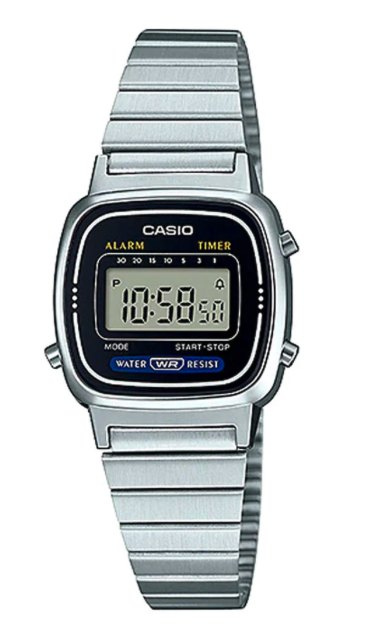
\includegraphics[width=2cm]{/Users/joaquin/Documents/GitHub/Ayudant-as-IO/Primavera 2024/A7/0.png}};
                \node at (10,0) [below] {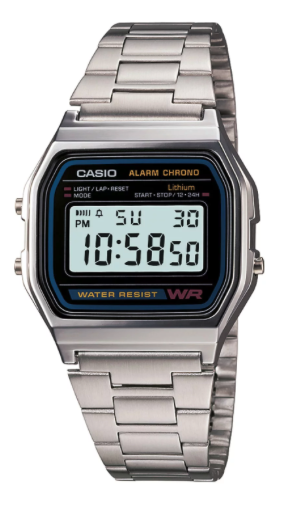
\includegraphics[width=2cm]{/Users/joaquin/Documents/GitHub/Ayudant-as-IO/Primavera 2024/A7/1.png}};
                
                % Dibuja las líneas verticales en 0 y 1
                \draw (0,0.1) -- (0,-0.1);
                \draw (10,0.1) -- (10,-0.1);
            \end{tikzpicture}
        \end{center}
        ¿Por qué una marca introduciría tantos relojes de calidades similares pero con aspectos distintos? pues porque darle en el gusto a las personas aumenta la disposición a pagar, y en caso de competencia puede aumentar el precio que se puede cobrar por sobre el costo marginal.
        
    \end{solution}

    \item[\textbf{e.}] Al diferenciarse verticalmente el producto cambia, por ejemplo añadiendo funciones o mejorando la calidad de los materiales. 
    \begin{solution}
        Verdadero. La diferenciación vertical cambia características del producto que inciden directamente en su calidad. Estos modelos se diferencian muy poco en aspecto, apuntan al mismo mercado, pero difieren en calidad de materiales y funcionalidades.
        \begin{center}
            \begin{tikzpicture}
                % Dibuja la línea horizontal
                \draw[blue, thick] (0,0) -- (10,0);
                
                % Coloca los puntos y las imágenes en los extremos
                \node at (0,0) [below] {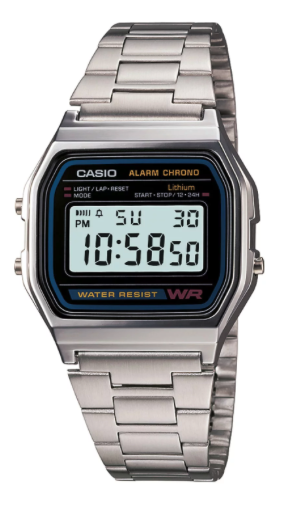
\includegraphics[width=2cm]{/Users/joaquin/Documents/GitHub/Ayudant-as-IO/Primavera 2024/A7/1.png}};
                \node at (10,0) [below] {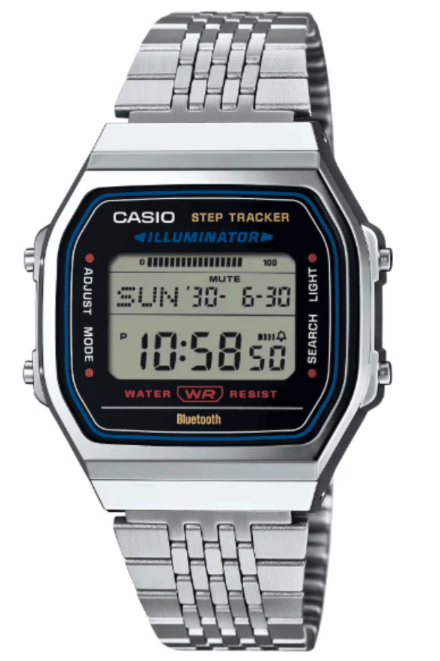
\includegraphics[width=2.25cm]{/Users/joaquin/Documents/GitHub/Ayudant-as-IO/Primavera 2024/A7/4.png}};
                
                % Coloca una imagen en el medio
                \node at (5,0) [below] {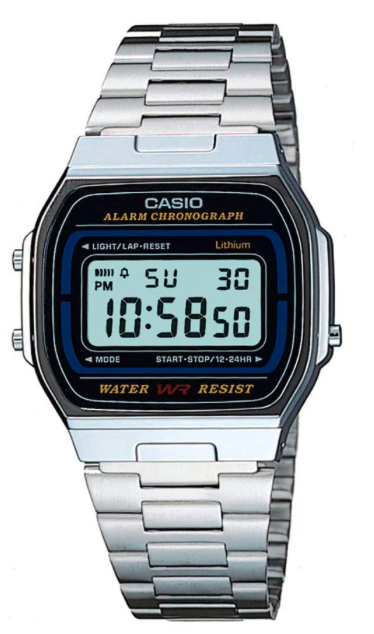
\includegraphics[width=2cm]{/Users/joaquin/Documents/GitHub/Ayudant-as-IO/Primavera 2024/A7/3.png}};
                
                % Dibuja las líneas verticales en 0, 5, y 10
                \draw (0,0.1) -- (0,-0.1);
                \draw (5,0.1) -- (5,-0.1);
                \draw (10,0.1) -- (10,-0.1);
                
                % Coloca los números arriba de cada línea vertical
                \node at (0,0.2) [above] {\$25.000};
                \node at (5,0.2) [above] {\$48.000};
                \node at (10,0.2) [above] {\$95.000};
                
            \end{tikzpicture}
        \end{center}
        ¿Por qué una marca introduciría tantos relojes de calidades distintas pero con aspectos similares? En un mismo mercado habrán personas que estarán más dispuestas que otras por pagar por calidad. Para obtener mayor excedente de estas personas se mejora la calidad del bien cobrando obvio un mayor precio.
        
    \end{solution}

    \item[\textbf{f.}] El modelo de Salop es lo mismo que el modelo de Hotelling pero asumiendo una ciudad circular.
    \begin{solution}
        Falso. El modelo de Salop tiene como objetivo entender la entrada de firmas. Se supone una ciudad circular para dar por sentado que no hay ubicaciones privilegiadas sobre otras, todas las empresas son equidistantes entre sí. 
        \begin{center}
            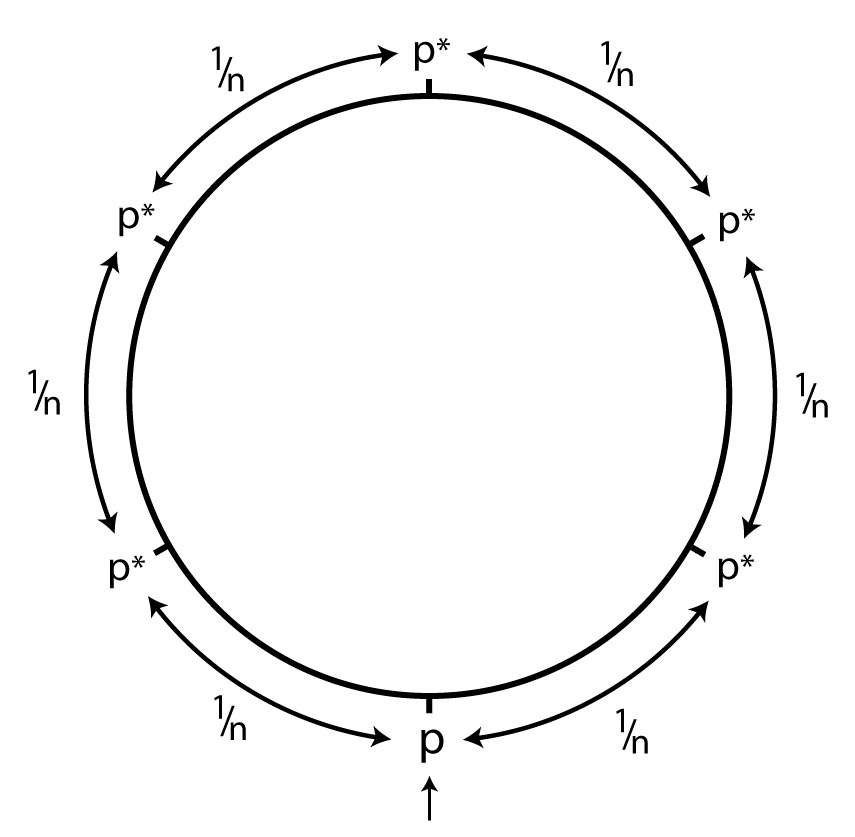
\includegraphics[width = 5.5cm]{/Users/joaquin/Documents/GitHub/Ayudant-as-IO/Primavera 2024/A7/Ciudad-circular-de-Salop.jpg}
        \end{center}
    \end{solution}
    \item[\textbf{g.}] En un modelo tipo Hotelling con decisiones de localización y luego competencia en precios, ¿Cuáles son las razones a favor y en contra de que las firmas produzcan bienes cada vez más diferenciados?
    \begin{solution}
        El efecto de demanda crea incentivos para que las firmas produzcan bienes con poca diferenciación. Cuando las empresas se acercan hacia el centro de la ciudad capturan mayor demanda.
        
        Sin embargo, el efecto estratégico nos dice que la competencia en precios en más fuerte cuanto menos diferenciados sean los bienes. Cuando las empresas se alejan del centro de la ciudad reducen la competencia por precios. 
    \end{solution}
\end{itemize}




\subsection{Diferenciación Horizontal Pura}
Considere una ciudad lineal que va de $0$ a $1$, dos empresas $L$ y $R$ deciden en que parte ubicarse, $\delta _L,\delta_R \in [0,1]$. Ambas ofrecen un productos homogéneos (son sustituibles) y se ofrecen a un precio $p_L, p_R$ según cada firma.\footnote{Lo único diferente de ambos productos son el lugar de la ciudad en que se venden.} Los potenciales consumidores de estas firmas se distribuyen de forma uniforme y los caracteriza la siguiente función de utilidad,
\begin{equation*}
    U_{ij} = \bar{u} + (y-p_j) - \theta (\delta_j - v_i)^2 \label{función utilidad}
\end{equation*}
\begin{enumerate}
    \item[\textbf{a.}] Explique cada parte de la función de utilidad y su interpretación intuitiva.
    \begin{solution}
        La función de utilidad es con respecto al individuo $i$ compradno a la firma $j$. En primer lugar $\bar{u}$ es una utilidad fija que les brinda el producto, $y-p_j$ es la utilidad neta de comprar el producto a la firma $j$. 

        Por último, $\theta(\delta_j - v_i)^2$ es el costo de transporte que incurre el individuo $i$ para comprarle a la firma $j$. 
    \end{solution}
    \item[\textbf{b.}] Cuántos individuos indiferentes hay en una ciudad lineal. Qué caracteriza a estos individuos. Encuentre su ubicación. 
    \begin{solution}
        En una ciudad lineal habrá un único individuo indiferente entre comprar a la firma $L$ o $R$. Este individuo es tal que $U_{\bar{i}L} = U_{\bar{i}R}$. Su ubicación la podemos encontrar planteando tal ecuación:
        \begin{align*}
    U_{iL} &= U_{iR} \\ 
    \bar{u} + (y-p_L) - \theta (\delta_L - \bar{v})^2 &= \bar{u} + (y-p_R) - \theta (\delta_R - \bar{v})^2 \\
    (p_R - p_L) - \theta (\delta _L ^2 - 2\delta_L \bar{v} + \bar{v}^2) &= - \theta (\delta_R^2-2\delta_R \bar{v} + \bar{v}^2 ) \\
    (p_R - p_L) - \theta \delta_L^2 + \theta \delta_R^2 &= 2\theta \delta _R \bar{v} - 2\theta \delta_L \bar{v}  \\
    (p_R - p_L) + \theta (\delta_R^2 - \delta_L^2 ) &= \bar{v} \cdot 2\theta (\delta _R - \delta_L) \\
    \bar{v} = \frac{p_R-p_L}{2\theta (\delta_R-\delta_L)} + \frac{\delta_R^2 -\delta _L^2}{2(\delta_R-\delta_L)} \\
    \xrightarrow{(a-b)(a+b)= a^2 - b^2} \frac{p_R-p_L}{2\theta (\delta_R-\delta_L)} + \frac{\delta_R + \delta_L}{2} \\
    \boxed{\bar{v} = \frac{p_R-p_L}{2\theta (\delta_R-\delta_L)} + \frac{\delta_R + \delta_L}{2}}
    \end{align*}

    \end{solution}
    \item[\textbf{c.}] Calcule las cuotas de mercado de ambas firmas. 
    \begin{solution}
        La cuota de mercado de la firma $L$ serán todos los individuos a la izquierda de $\bar{v}$ y $R$ se queda con el resto del mercado $1-\bar{v}$.

\begin{align*}
    D_L(p,\delta;\theta) &= \bar{v} = \frac{p_R-p_L}{2\theta (\delta_R-\delta_L)} + \frac{\delta_R + \delta_L}{2} \\
    D_R(p,\delta;\theta) &= 1 - \bar{v} = 1 -  \frac{p_R-p_L}{2\theta (\delta_R-\delta_L)} - \frac{\delta_R + \delta_L}{2} 
\end{align*}
    \end{solution}
    En el modelo de Hotelling las firmas en un primer turno eligen donde ubicarse en la ciudad para luego en un segundo empezar a vender a un cierto precio. 
    \item[\textbf{d.}] Suponga que bajo un nuevo marco legal el precio del producto está fijado. ¿Donde les conviene ubicarse las firmas?
    \begin{solution}
        Dado que las firmas están obligadas a poner un nuevo precio, dada la ubicación de la competencia la mejor respuesta siempre será estar un $\varepsilon$ más cerca del centro ($0,5$). El equilibrio será $\delta_R = \delta_L = 0,5$.

        Aquí estamos frente a un caso de mínima diferenciación. Como los precios están dados las firmas intentarán maximizar su cuota de mercado mediante su ubicación. 

        Puede ver que si $p_R = p_L $ y $\delta_R = \delta_L = 0,5$ en las funciones de demanda $D_L(p,\delta;\theta),D_R(p,\delta;\theta)$ la demanda de cada una es $0,5$, se reparten el mercado en partes iguales.
    \end{solution}
    \item[\textbf{e.}] Ahora volvamos al escenario sin el marco regulatorio, las firmas eligen sus precios. Encuentre las funciones de reacción de ambas firmas. Encuentre el equilibrio de Nash.
    \begin{solution}
        Hacemos un cambio de variable para hacer la matemática más fácil.
\begin{align*}
    \theta(\delta_R-\delta_L) = t \\
    \frac{\delta_R+\delta_L}{2} = \tau
\end{align*}
Para la empresa $L$.
\begin{align*}
    \max_{p_L} \quad \Pi_L &= (p_L - c) \left( 
 \frac{p_R-p_L+2\tau t}{2t}  \right) \\
    & = \frac{p_Lp_R - p_L^2 +2\tau tp_L}{2t} + \frac{p_Lc-p_Rc-2\tau t c}{2t} \\
    \frac{\partial \Pi_L}{\partial p_L} & = \frac{p_R-2p_L+2\tau t +c}{2t} = 0 \\
    & = p_R -2p_L+2\tau t +c = 0 \\
    & \quad \\
    & \boxed{p_L = \frac{1}{2} (p_R + c) + \tau t} 
\end{align*}

Para la empresa $R$.
\begin{align*}
    \max_{p_R} \quad \Pi_R &= (p_R-c) \left( \frac{p_L-p_R +2t -2t\tau}{2t}   \right) \\
    & = \frac{p_Rp_L - p_R^2 +2tp_R-2t\tau p_R}{2t} - c \frac{p_L-p_R +2t -2t\tau}{2t} \\
    \frac{\partial \Pi_R}{\partial p_R} & = p_L -2p_R+2t-2t\tau +c = 0 \\
    & \boxed{p_R = \frac{1}{2}(p_L + c) + t(1-\tau)}
\end{align*}

Reemplazando las simplificaciones que hicimos tendríamos esta función de reacción para la firma $L$.
\begin{align*}
    p_L^* = \frac{1}{2}(p_R+c) + \frac{\theta(\delta_R^2 -\delta_L^2)}{2}
\end{align*}
Siempre que las firmas estén a una misma distancia del centro $p_L = p_R$, por lo que podemos reemplazar para obtener el equilibrio de nash. 
\begin{equation*}
    p = c + \theta(\delta_R - \delta_L)
\end{equation*}
    \end{solution}
    \item[\textbf{f.}] Grafique las funciones de reacción. Muestre como se mueven las curvas al cambiar los costos de transporte.  
    \begin{solution}
        \textbf{ \href{https://www.geogebra.org/calculator/bv9nzjae}{\underline{Link}}}
    \end{solution}
    \item[\textbf{g.}] Supongamos que usted es un planificador social omnipotente que busca maximizar el bienestar de los consumidores. Cómo cree que debiesen ubicarse las firmas.
    \begin{solution}
        La solución socialmente óptima es la que minimiza los costes de transporte y sería $\delta_L=1/4$ y $\delta_R=3/4$. Por tanto desde el punto de vista social hay demasiada diferenciación del producto cuando el mercado es privado.
    \end{solution}
\end{enumerate}

\subsection{Diferenciación Vertical Pura}

Ahora considere que las empresas no se distinguen en características horizontales de los productos pero pueden decidir en el primer turno la calidad de su producto y en el segundo competir por precios. \vspace{3mm}

Podríamos imaginar una distribución lineal de calidad del producto, donde 1 es la máxima calidad y 0 la mínima. La empresa de menor calidad se ubicaría en $b$ mientras que la de mayor calidad se ubicaría en $g$, por lo que se acaba de explicar $b<g$.

\begin{center}
    \begin{tikzpicture}
        % Dibuja la línea
        \draw[blue, thick] (0,0) -- (4,0);
        
        % Coloca los puntos y las etiquetas
        \node at (0,0) [below] {\textit{\textbf{0}}};
        \node at (4,0) [below] {\textit{\textbf{1}}};
        
        % Coloca las etiquetas a y b
        \node at (1.5,-0.065) [below] {b};
        \node at (2.5,-0.090) [below] {g};
        
        % Dibuja las líneas verticales en a y b
        \draw (1.5,0.1) -- (1.5,-0.1);
        \draw (2.5,0.1) -- (2.5,-0.1);
    \end{tikzpicture}
\end{center}


Considere un individuo con una utilidad $U_x^i(p_i)$, siendo $x$ la posición del individuo (su disposición a pagar por calidad) e $i = b,g$ la empresa a la que le compra. 
\[
U_x^i (p_i) = 
\begin{cases} 
bx - p_b & \text{si } i = b \\
gx - p_g & \text{si } i = g 
\end{cases}
\]

\begin{itemize}
    \item[\textbf{a.}] ¿Cuál es el procedimiento para resolver este tipo de juego?
    \begin{solution}
        Estos juegos por turnos se resuelven por inducción para poder encontrar un equilibrio de nash consistente con individuos que elijen su mejor respuesta mirando hacia el futuro. Es decir tienen que ver hacia el futuro y pensar en el precio que deberían poner dada las ubicaciones en calidad. Para luego elegir las ubicaciones que tomarían. 

        De lo contrario, si eligieran una ubicación sin pensar en la pelea por precios que habría posteriormente puede que lleguemos a un equilibrio de nash (dadas las funciones de reacción de precios) que no sea consitente con individuos racionales que miran hacia al futuro. 
    \end{solution}
    \item[\textbf{b.}] Encuentre el punto $\hat{x}$ en que se encuentra el consumidor indiferente. Demuestre que comprar calidad hace más felices a los dispuestos a pagar por calidad que los que no valoran tanto la calidad.
    \begin{solution}
        \begin{align}
            U_{\hat{x}}^b(p_b) = U_{\hat{x}}^g(p_g) \notag \\
            b\hat{x} - p_b =  g\hat{x} - p_g \notag \\
            \hat{x} (b-g) = p_b-p_g \notag \\
            \boxed{\hat{x} = \frac{p_g-p_b}{g-b}} \label{ind indife}
        \end{align}
        Para ver que comprar calidad hace más felices a los dispuestos a pagar por calidad que los que no valoran tanto la calidad podemos evaluar la diferencia. 
        \begin{align*}
            U_{\hat{x} + \varepsilon}^{b}(p_b) - U_{\hat{x} + \varepsilon}^{g}(p_g) < 0 , \quad \varepsilon > 0 \\
            b(\hat{x} + \varepsilon) - p_b - g(\hat{x} + \varepsilon) + p_g \\
            \underbrace{b\hat{x} - p_b -  g\hat{x} + p_g }_{= 0} + b\varepsilon - g\varepsilon \\
            \boxed{-(g-b)\varepsilon < 0 }
        \end{align*}
    \end{solution}
    \item[\textbf{c.}] Grafique las funciones de utilidad en función de la calidad para individuos sujeto a que si compran $g$ o $b$. 
    \begin{solution}
        \begin{center}
            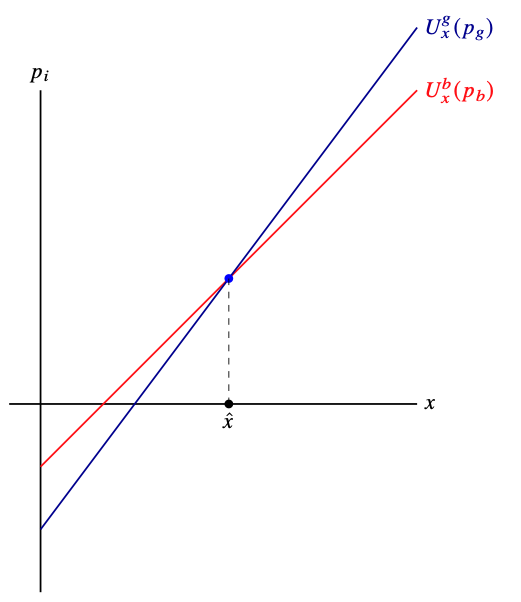
\includegraphics[width = 5.5cm]{/Users/joaquin/Documents/GitHub/Ayudant-as-IO/Primavera 2024/A7/utildiades vertical.png}
        \end{center}
    \end{solution}
    \item[\textbf{d.}] Encuentre las funciones de reacción de las firmas dadas las ubicaciones. Suponga que no hay costos marginales. 
    \begin{solution}
        Las ubicaciones estarán dadas, tenemos la información del individuo indiferente por lo cual podemos expresar las funciones de reacción de precios en función del precio de la competencia sujeta a las ubicaciones que se hayan tomado. \vspace{3mm}

        La demanda por los bienes de la empresa en $b$ estará dada por los que estén a la izquierda de $\hat{x}$, por lo que $b$ maximiza lo siguiente.
        \begin{align*}
            \max_{p_b} \quad \pi_b(p_g;g,b) = p_b \hat{x} = p_b\frac{p_g-p_b}{g-b}
        \end{align*}
        Derivamos las condiciones de primer orden con tal de encontrar la función de reacción despejando $p_b$ de la derivada.
        \begin{align*}
            \frac{\partial \pi_b}{p_b} = - 2\frac{p_b}{g-b} + \frac{p_g}{g-b} = 0 \\
            \boxed{p_b = \frac{1}{2}p_g} 
        \end{align*}
        Es decir que dadas las diferencias en calidad el productor del producto de menor calidad fijará la mitad de precio que el otro. Por otro lado esta ecuación se mantiene cuando no hay mínima diferenciación, es decir tenemos $g\neq b$. 

        Ahora para sacar la función de reacción de $g$ es análogo. 
        \begin{align*}
            \max_{p_g} \quad \pi _g (p_b;g,b) =p_g (1-\hat{x}) = p_g \left( 1 - \frac{p_g-p_b}{g-b}\right) \\
            \frac{\partial \pi_g}{\partial p_g} = 1 - 2\frac{p_g}{g-b} + \frac{p_b}{g-b} = 0 \\
            \boxed{p_g = \frac{(g-b)+p_b}{2}}
        \end{align*}
    \end{solution}
    \item[\textbf{e.}] Encuentre el equilibrio de Nash con las funciones de reacción que encontró en el ítem anterior. 
    \begin{align*}
        p_b(p_g) = \frac{1}{2}p_g, \qquad p_g(p_b) = \frac{(g-b)+p_b}{2}
    \end{align*}
    \begin{solution}
        Encontremos el precio de la firma de relativa menor calidad.
        \begin{align*}
            p_b &= \frac{1}{2}\times \frac{(g-b)+p_b}{2}   = \frac{(g-b)+p_b}{4} \\
            p_b \times \frac{3}{4} &= \frac{g-b}{4} \\
            &\boxed{p_b = \frac{1}{3}(g-b)}
        \end{align*}
        Entonces podemos obtener directamente el precio de la firma de mayor calidad.
        \begin{align*}
            p_g &= \frac{(g-b)}{2} +  \frac{1}{2} \times  \frac{1}{3}(g-b) \\
            &= \frac{1}{2}(p-g) +  \frac{1}{6}(p-g) \\
            &\boxed{p_g = \frac{2}{3}(g-b)}
        \end{align*}
        La empresa con más alta calidad cobra un precio superior pero ambas empresas colocan un precio por encima del coste marginal. Es decir, relajaron la competencia diferenciandose por lo que obtendrán beneficios.
    \end{solution}
    \item[\textbf{f.}] Encuentre la demanda y beneficios en el equilibrio.
    \begin{solution}
        La demanda por las firmas dependía del individuo indiferente que a su vez dependía de los precios dadas las ubicaciones. Ahora que tenemos los precios dadas las ubicaciones podemos obtener la demanda reemplazando $\hat{x}$. \vspace{3mm}

        Demanda de $b$.
        \begin{align*}
            \hat{x} = \frac{p_g-p_b}{g-b} = \frac{\left(\frac{2}{3}(g-b) -  \frac{1}{3}(g-b) \right)}{g-b} = \frac{\frac{1}{3}(g-b)}{g-b} = \frac{1}{3}\\
        \end{align*}
        Por tanto la demanda de $g$ son $2/3$.

        Entonces los beneficios de $\pi_b$ son,
        \begin{align*}
            \pi_b &= p_b \hat{x} = \frac{1}{3}(g-b) \times \frac{1}{3} \\
            & \boxed{\pi_b = \frac{1}{9} (g-b)}
        \end{align*}
        De la misma manera encontramos los beneficios de la empresa de relativa mayor calidad.
        \begin{align*}
            \pi_g &= p_g(1-\hat{x}) =\frac{2}{3}(g-b) \times \frac{2}{3}\\
            & \boxed{\pi_g = \frac{4}{9}(g-b)}
        \end{align*}
    \end{solution}
\item[\textbf{g.}] Encuentre las ubicaciones que le conviene a las firmas para maximizar sus beneficios. ¿Le conviene centrarse o diferenciarse? 
\begin{solution}
    Por fin llegamos al primer turno. Donde dados los beneficios que están en función de las ubicaciones se puede obtener la ubicación de cada empresa que maximiza los beneficios. 
    \begin{align*}
        \max_{b} \quad \pi_b = \frac{1}{9} (g-b)
    \end{align*}
    La derivada es negativa, hay que producir con muy baja calidad posible, $b = 0$. Para el caso de la firma de mayor calidad relativa. 
    \begin{align*}
        \max_g \quad \pi_g = \frac{4}{9}(g-b)
    \end{align*}
    Maximizamos aumentando $g$ por sobre lo máximo posible, entonces $g=1$.

    Acabamos encontrar que las firmas se diferenciarán lo máximo posible para maximizar los beneficios. Una firma producirá la mayor calidad posible y otra la menor calidad posible, ¡aún cuando sean igual de baratos de producir! ($c= 0$)
\end{solution}
\end{itemize}

\newpage

\section*{Propuestos de discriminación de precios}

\subsection*{Comentes}

\begin{itemize}
    \item[\textbf{a.}] ¿Cuál es la diferencia entre discriminación de primer y tercer grado?
    \item[\textbf{b.}] Caracterice los mercados en los que suele haber discriminación de primer grado y tercer grado. 
    \item[\textbf{c.}] Es imposible que una firma monopólica logre captar todo el excedente del consumidor, puesto que los precios y la estrategia que impongan dependerán también de factores como la elasticidad de la demanda.
    \item[\textbf{d.}] ¿Discriminar o no discriminar? Discuta los principios básicos para responder esta pregunta.
    \end{itemize}

\subsection*{Matemático: Discriminación de tercer grado}

En un pueblo del sur de Chile hay un único museo recibe a visitantes nacionales y extranjeros, quienes presentan una mayor valoración del museo. El costo marginal de producción del museo es 1 por cada visitante y no hay costos fijos. Las demandas de extranjeros y nacionales será,
\begin{align*}
    Q_E = 10-P_E \\
    Q_N = 8 - P_N
\end{align*}
\begin{itemize}
    \item[\textbf{a.}] Suponga uqe el museo monopólico fija un precio uniforme, ¿Qué precio cobra y qué beneficio obtiene? ¿Qué condición debe cumplirse para que se venda a ambos grupos?
    \item[\textbf{b.}] Suponga ahora que el monopolio puede discriminar en tercer grado. Calcule los precios de cada mercado y los beneficios del museo.
    \item[\textbf{c.}] Un compañero le menciona que el museo debería enfocarse solo en el grupo de alta valoración. Demuéstrele al compañero que al museo no le conviene enfocarse solo en una parte del mercado, cuando tiene la opción de discriminar precios. 
    \item[\textbf{d.}] Comparando los beneficios del monopolio con la estrategia de precio uniforme y de discriminación ¿Cuál le conviene más? Además, calcule los excedentes de los consumidores extranjeros y nacionales ¿Cuál grupo se beneficia de la discriminación de tercer y cuál se perjudica?
    \item[\textbf{e.}] ¿Qué pasa con el beneficio social? Calcule también el producto total ofrecido en cada estrategia y comente su relación con los cambios en bienestar o ineficiencias que puedan estar ocurriendo. ¿Qué otros factores explican los cambios en bienestar al pasar de una estrategia a otra?
\end{itemize}

\end{document}
